%
% Ricci-Krümmung
%
\section{Ricci-Krümmung
\label{buch:kruemmung:section:ricci}}
\kopfrechts{Ricci-Krümmung}
%
% fig-schnittkruemmung.tex
%
% (c) 2025 Prof Dr Andreas Müller
%
\begin{figure}
\centering
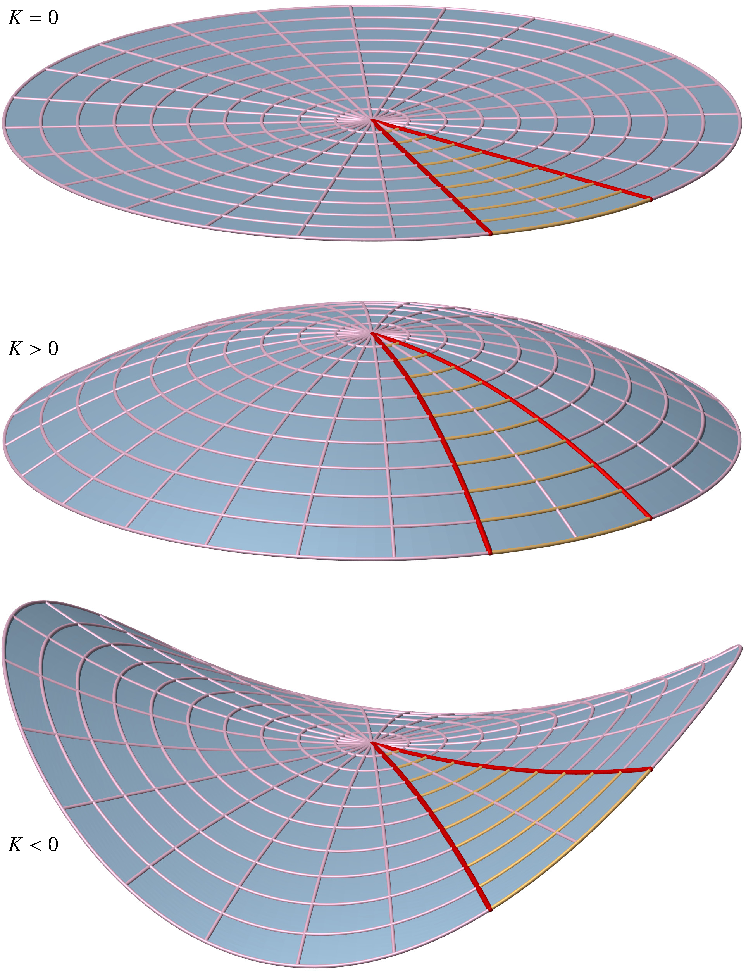
\includegraphics{chapters/110-kruemmung/images/kruemmung.pdf}
\caption{Die Schnittkrümmung bestimmt, wie schnell sich Geodäten
voneinander entfernen.
Der Abstand der Geodäten wächst linear mit dem Radius, wenn 
$K=0$ ist, der Abstand wächst schneller als linear für $K<0$ und
langsamer als linear für $K>0$.
\label{buch:kruemmung:fig:schnittkruemung}}
\end{figure}

Die Komponente $R^l\mathstrut_{ijk}$  des Riemann-Krümmungstensors
beschreibt, wie sich die $l$-Komponente des des $i$-ten 
Standardbasisvektors $\vec{e}_i$ beim Paralleltransport um
ein infinitesmales Quadrat mit dem 2-Vektor $\vec{e}_j\wedge \vec{e}_k$
verändert.
Für die physikalische Interpretation des Gravitationsfeldes ist
es wichtig zu verstehen, wie sich der Abstand von Geodäten mit
ähnlichen Anfangsbedingungen verändert, da wir dies als relative
Beschleunigung und damit als Anziehungs- oder Abstossungskraft 
interpretieren können.

%
% Schnittkrümmung
%
\subsection{Schnittkrümmung}
Wir betrachten zwei Geodäten mit initialem Tangentialvektor
$\vec{v}$, deren Anfangspunkte sich um eine kleine Verschiebung
in Richtung des Tangentialvektors $\vec{s}$ unterscheiden.

\begin{lemma}
Für die kovariante Ableitung zum Levi-Cività-Zusammenhang gilt
\[
\nabla_{\vec{v}}\nabla_{\vec{s}}\vec{v}
=
\nabla_{\vec{v}}\nabla_{\vec{v}}\vec{s}.
\]
\end{lemma}

\begin{proof}
Wir berechnen in Komponenten
Die Komponenten der Ableitungen der ersten kovarianten Ableitungen
sind
\begin{align*}
(\nabla_{\vec{s}}\vec{v})^i
&=
\biggl(
\frac{\partial v^i}{\partial x^k}
-
\Gamma^i_{kl} v^l
\biggr)
s^k
\\
(\nabla_{\vec{v}}\vec{s})^i
&=
\biggl(
\frac{\partial s^i}{\partial x^k}
-
\Gamma^i_{kl} s^l
\biggr)
v^k
\end{align*}

\end{proof}

\begin{align*}
\nabla_{\vec{v}}\nabla_{\vec{v}}\vec{s}
&=
-R(\vec{s}\wedge\vec{v})\cdot \vec{v}
\end{align*}
d.~h.~der Krümmungstensor gibt an, wie sich der
Verschiebungsvektor $\vec{s}$ zwischen den Geodäten ändert.

%
% Ricci-Krümmung
%
\subsection{Ricci-Krümmung}
Das Skalarprodukt
\begin{equation}
R(\vec{v},\vec{s})(\vec{v})\cdot\vec{s}
=
\langle
R(\vec{v}\wedge\vec{s})(\vec{v}) ,\vec{s}
\rangle_g
\label{buch:kruemmung:ricci:eqn:Rvsvs}
\end{equation}
ist ein Mass für die Änderung des Abstandes der Geodäten.
Es ist linear in allen Vektoren.
Aus den Symmetrieeigenschaften des riemannschen Krümmungstensors folgt
auch, dass es nur von $\vec{v}\wedge\vec{s}$ abhängt.
Multipliziert man $\vec{v}$ oder $\vec{s}$ mit einem Faktor $\lambda$,
wird  der Ausdruck \eqref{buch:kruemmung:ricci:eqn:Rvsvs} mit
$\lambda^2$, multipliziert.
Insbesondere ist
\[
K(\vec{s},\vec{v})
=
\frac{R(\vec{v}\wedge\vec{s})(\vec{v})\cdot\vec{s}}{|\vec{v}\wedge\vec{s}|^2}
\]
unabhängig von der Länge von $\vec{v}$ und $\vec{s}$.
Sie heisst die Schnittkrümmung.
Sie ist postiiv, wenn sich die Geodäten nähern und negativ, wenn sie
sich entfernen.

Ist $X$ ein Vektor mit den Komponenten $X^i$, dann ist
\[
R(\vec{e}_j\wedge X)(X)\cdot e_l
=
R^l\mathstrut_{ijk}X^iX^k.
\]
Für $l=j$ ergibt sich die Schnittkrümmung in der $\vec{e}_j$-$X$-Ebene.
Sie gibt die Änderung des Abstandes der Geodäten mit
Anfangsvektor $X$ an, wenn man den Anfangspunkt infinitesmal in
$\vec{e}_j$-Richtung verschiebt.

Die Summe
\begin{equation}
\sum_{j=1}^n
R(\vec{e}_j\wedge X)(X)\cdot \vec{e}_j
=
R^j\mathstrut_{ijk} X^iY^k
\label{buch:kruemmung:ricci:eqn:ricci}
\end{equation}
ist bis auf den Faktor $\frac1n$ der Mittelwert der Schnittkrümmungen
für die verschiedenen Differenzvektoren $\vec{s}=\vec{e}_j$.

\begin{definition}[Ricci-Krümmung]
\label{buch:kruemmung:ricci:def:ricci-kruemmung}
Der Tensor mit den Komponenten $R_{ik}=R^j\mathstrut_{ijk}$ heisst
der {\em Ricci-Krümmungstensor}.
Die Ricci-Krümmung zum Vektor $X$ ist
\[
\operatorname{Ric}(X,X)
=
\sum_{i,k=1}^n
\operatorname{Ric}(e_i,e_k)X^iX^k
=
R_{ik}X^iX^k.
\]
Sie ist eine quadratischer Form von $X$.
\end{definition}

Aus den Symmetrieeigenschaften des riemannschen Krümmungstensors folgt,
dass der Ricci-Tensor symmetrisch ist.

Die Konstruktion von $\operatorname{Ric}(X,X)$ als Summe über alle
Basisrichtungen ist ein richtungsunabhängiges Mass für die
Krümmung.
Positive Krümmung bedeutet, dass sich Geodäten im Mittel annähern.
Wir werden dies als gravitationelle Anziehungskraft interpretieren.
Wenn der Ricci-Tensor verschwindet, gibt es auch keine Gravitationskräfte.
Wir erwarten daher, dass es eine Feldgleichung gibt, die Masse und
Energie im Universum mit dem etwas spezielleren Ricci-Tensor verknüpft,
nicht mit dem ganz allgemeinen riemannschen Tensor.

%
% Krümmungsskalar
%
\subsection{Krümmungsskalar}
Die Spur des Ricci-Tensors
\[
R
=
g^{ik}R_{ik}
=
R^i_k
\]
heisst der {\em Krümmungsskalar}.
\index{Krummungsskalar@Krümmungsskalar}
Der Krümmungsskalar ist also Tensor nullter Stufe eine weitere Invariante,
die in einer Feldgleichung für die Gravitation vorkommen könnte.
